\section{PROPOSED FRAMEWORK (MAUI) BASED ON BOOLEAN SATISFIABILITY (SAT)}
\label{sec:framework}
In the proposed framework, aging tolerance is achieved by assigning specific/beneficial slacks into the designs, based on the following two idea and timing borrowing: ($i$) Aging manipulation on clock paths: The beneficial slacks is progressively created by different aging behaviors of the two clock paths $C_{i}$ and $C_{j}$, due to the different duty cycles of clock signal caused by DCCs. ($ii$) $V_{th}^h$ assignment for clock buffers: The beneficial slack is created by assigning the $V_{th}$ of certain clock buffers to high counterpart. In this way, clock latency is changed and thus give us an opportunity to further improve the aging tolerability of designs.

The overall flow of the proposed framework is depicted in Figure~\ref{fig:flow}, where we focus the following two issues:
\begin{enumerate}[leftmargin=*]
	\item \textbf{Minimization of clock period:} The clock period can be minimized since the performance degradation of the logic circuit is \enquote{tolerated} as a result of useful clock skews. The minimum required clock period thus implies maximum level of aging tolerance. As depicted in Figure~\ref{fig:flow}, a binary search for optimal clock period is involved in the proposed framework.
	\item \textbf{DCC deployment and selection of $V_{th}^h$ buffer leaders:} The problem of  DCC deployment and  selection of $V_{th}^h$ buffer leaders is formulated as a Boolean Satisfiability (SAT) problem. Therefore, the key of our framework is to represent the problem in \textit{conjunctive normal form} (CNF). A CNF representation is a conjunction of one or more clauses, where each clause is a disjunction of one or more Boolean variables. Thanks to the efficiency of existing SAT solver, the solution can be obtained efficiently. The end result of this formulation is the locations (in the existing clock tree) of DCCs and $V_{th}^h$ buffer leaders, such that when aging-induced clock skews are considered, the required clock period of the given circuit under $n$-year BTI is minimized. 
\end{enumerate}
%(1) 2018DATE
%Our proposed framework for aging tolerance is based on the two idea with the concept of time borrowing, so as to mitigate the aging-induced performance degradation of logic network. The first idea is to insert \textit{duty-cycle converters} (DCCs) in the existing clock tree, and the second idea is to assign the $V_{th}$ of certain clock buffers to high $V_{th}$ (i.e., $V_{th}^h$), by selecting $V_{th}^h$ buffer leaders from the existing clock buffers. In this way, we can intentionally create specific clock skews, compensating for the performance degradation of the logic circuit based on time borrowing. 

%We formulate the problem using Boolean satisfiability (SAT) and thanks to the efficiency of existing SAT solvers, the optimal solution can be obtained efficiently. The end result of this formulation is the locations (in the existing clock tree) of DCCs and $V_{th}^h$ buffer leaders, such that when aging-induced  clock skews are considered, the required clock period of the given circuit under $n$-year BTI is minimized. The clock period can be minimized since the performance degradation of the logic circuit is \enquote{tolerated} as a result of useful (aging-induced) clock skews. The minimum required clock period thus implies maximum level of aging tolerance. Note that, as mentioned in \ref{sec:mot:exp2}, $V_{th}^h$ buffer leader is an imaginary location instead of a physical gate such as DCC. It indicates the location where we begin assigning high $V_{th}$ to clock buffers toward flip-flops, excluding flip-flops.

%(1) DATE 2018
\begin{comment}
The basic idea of our MAUI framework for aging tolerance is to insert \textit{duty-cycle converters} (DCCs) in the existing clock tree, so as to intentionally create aging-induced clock skews which can compensate for the performance degradation of the logic circuit based on time borrowing. We formulate the problem using Boolean satisfiability (SAT) and thanks to the efficiency of existing SAT solvers, the optimal solution can be obtained efficiently. The end result of this formulation is the locations (in the existing clock tree) to insert DCCs such that, when aging-induced clock skews are considered, the required clock period of the given circuit under $n$-year BTI is minimized. Note that the clock period can be minimized since the performance degradation of the logic circuit is \enquote{tolerated} as a result of useful aging-induced clock skews. The minimum required clock period thus implies maximum level of aging tolerance.
\end{comment}

\begin{figure}
	\centering
	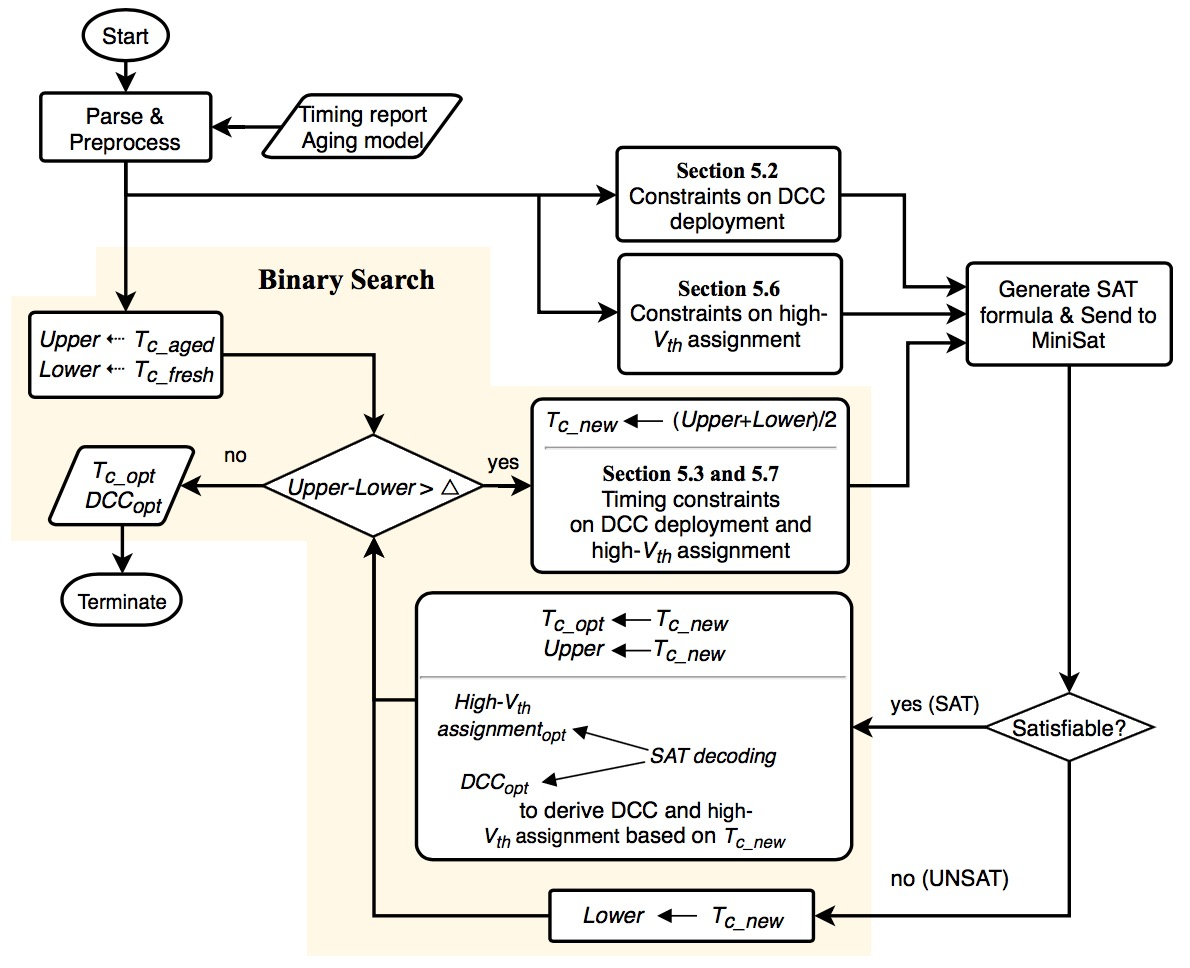
\includegraphics[width=1.0\columnwidth]{Flow_chart.png}
	\caption{The overall flow of MAUI}
	\label{fig:flow}
\end{figure}
 

The section is organized as follows: Section~\ref{subsec:eddcd} explains how the proposed problem of DCC deployment/insertion and leader selection are encoded by Boolean variables. Section~\ref{subsec:dccccc} and Section~\ref{subsec:tccc} describe three major components, DCC constraints, leader constraints and timing constraints, for our SAT-based formulation and how they are translated into legal SAT formula, i.e., CNF representation. Finally, we detail the timing model of aging (BTI degradation) prediction and $V_{th}^h$ buffers.

\afterpage{
\begin{figure}
	\centering
	%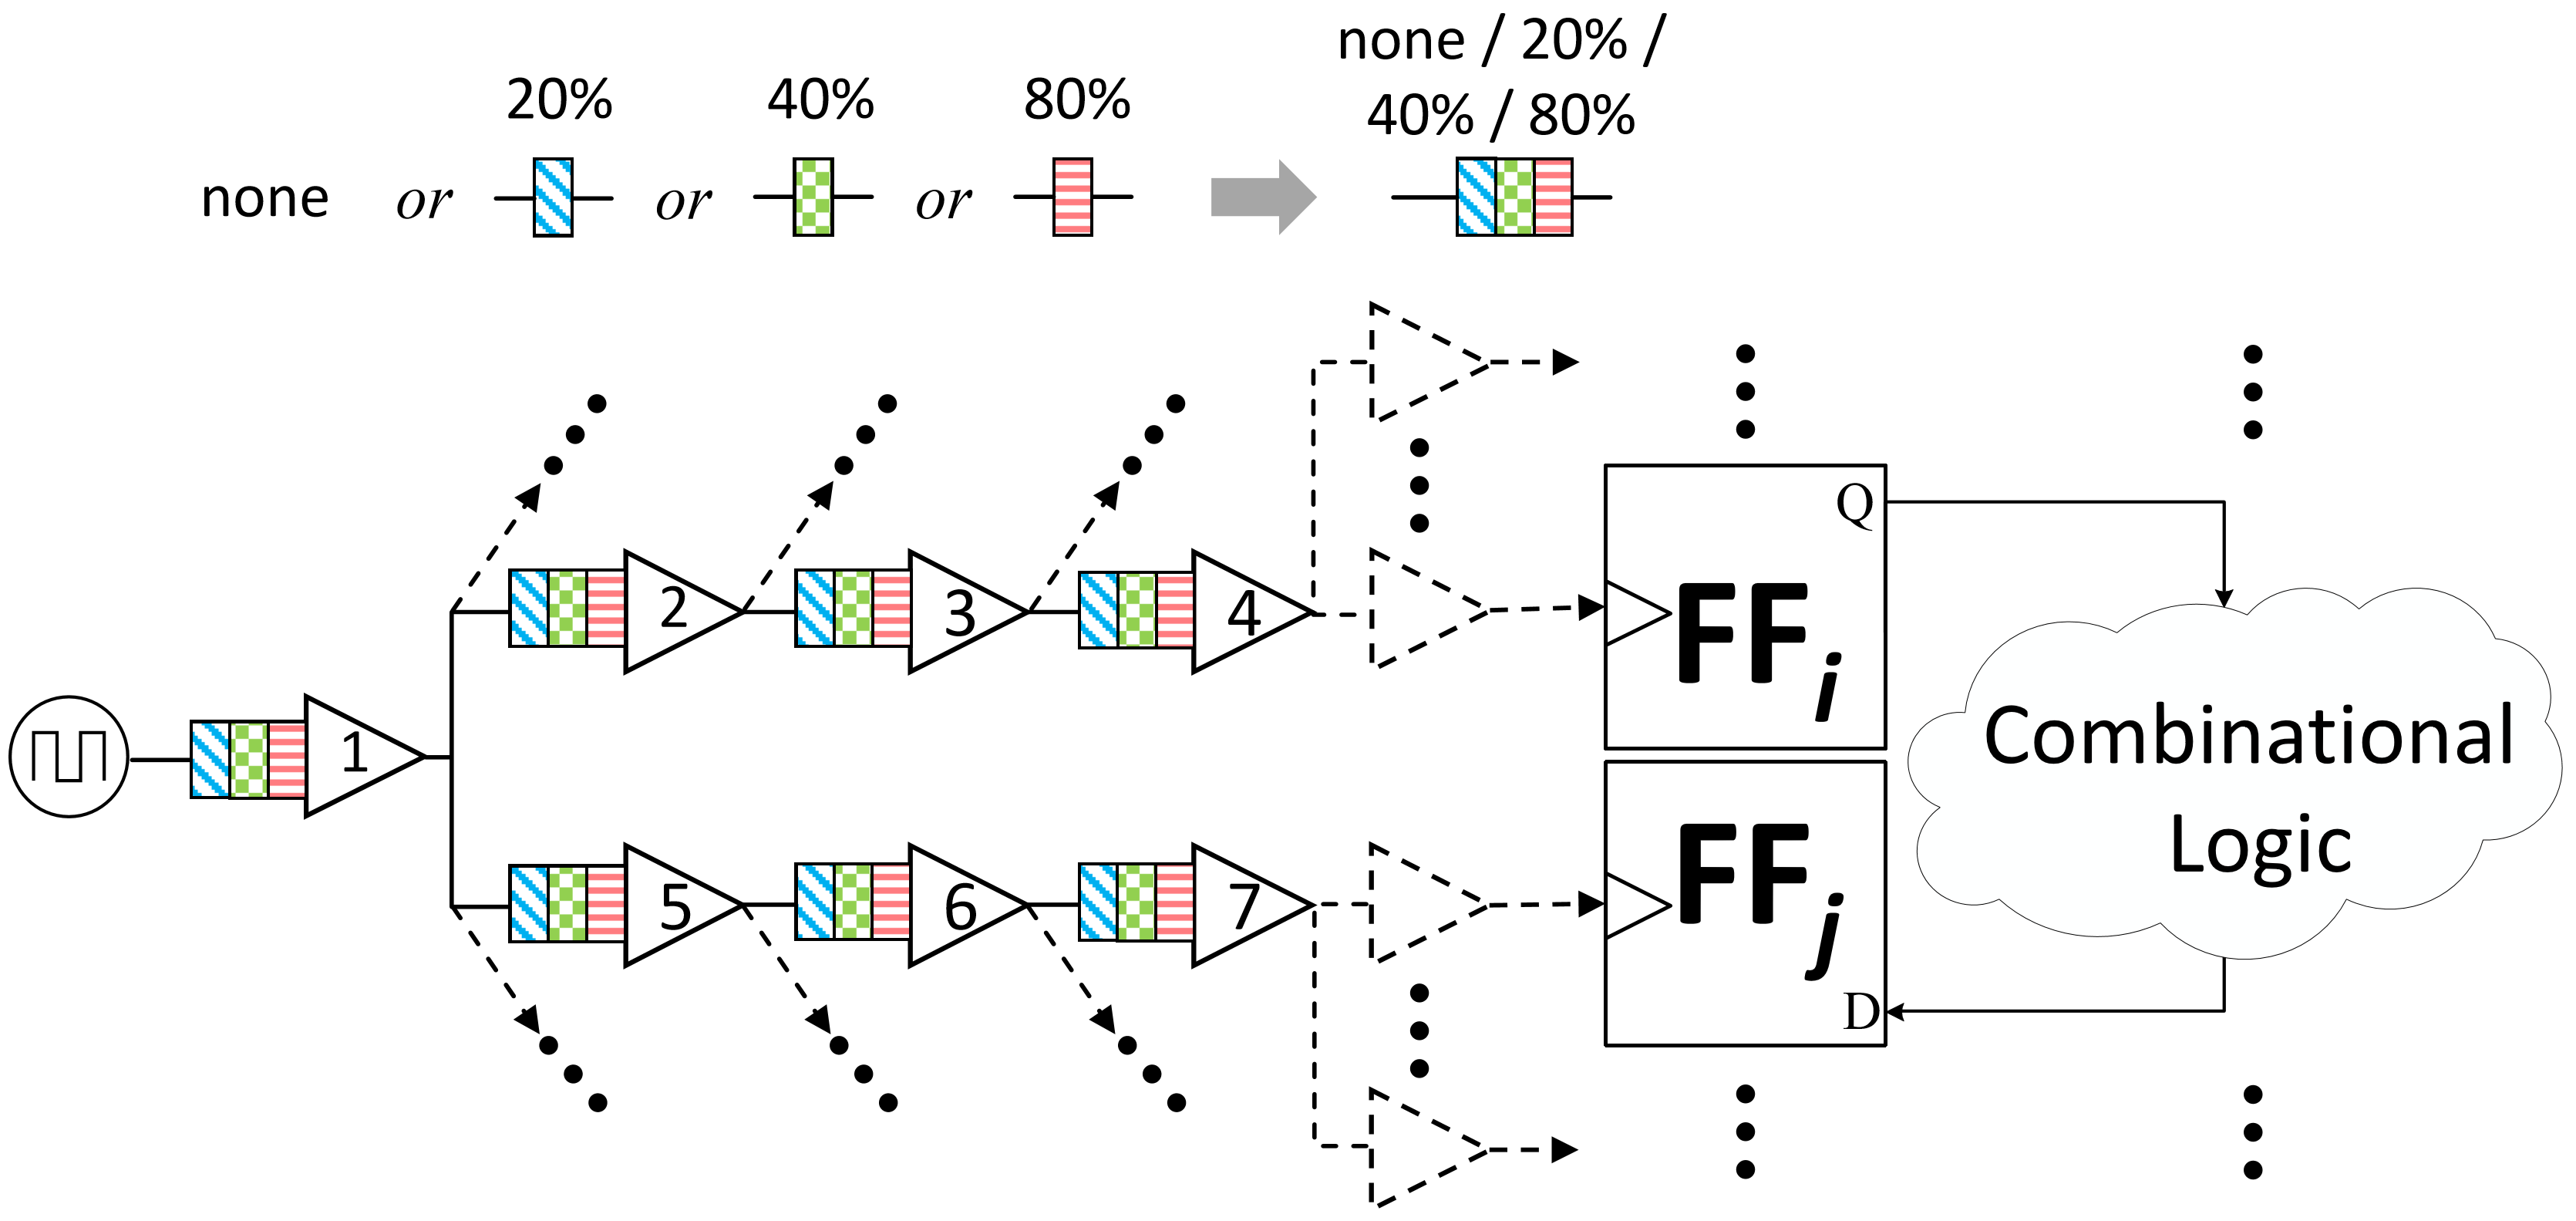
\includegraphics[width=0.9\columnwidth]{All_types_of_DCCs.png}
	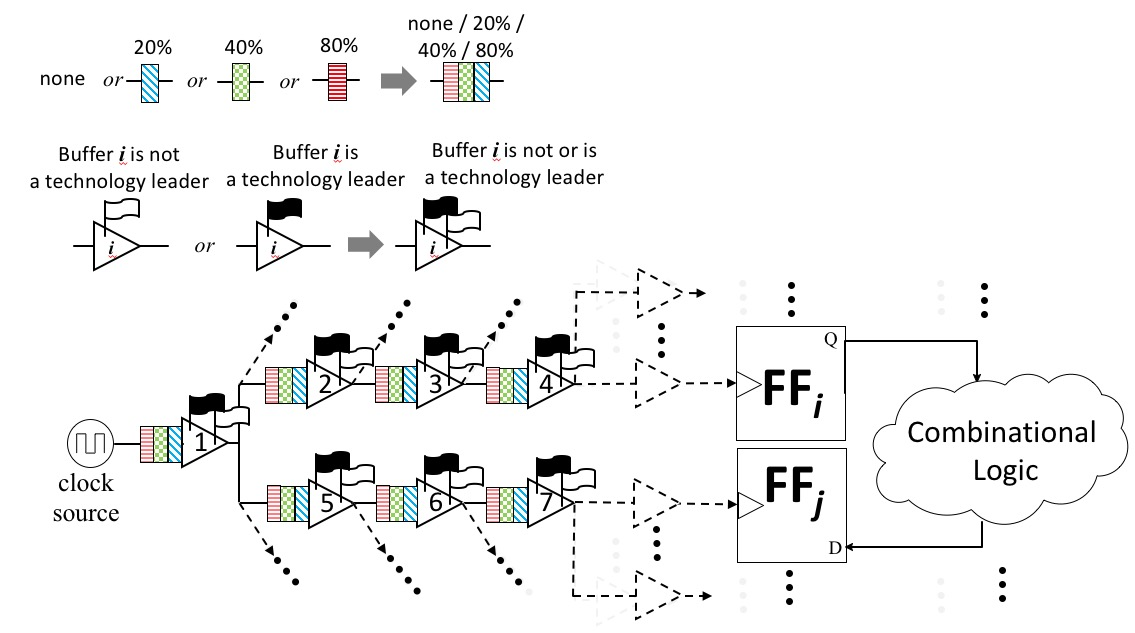
\includegraphics[width=1.0\columnwidth]{All_types_of_DCCs_and_leaders.png}
	\caption{Generalized DCC insertion and $V_{th}^h$ buffer leader selection, for a target pair of flip-flops}
	\label{fig:dcctype}
\end{figure}
}

%(3) DATE 2018
\subsection{Encoding for DCC Deployment and $V_{th}^h$ Buffer Leader Selection}
\label{subsec:eddcd}
The problem of DCC deployment and leader selection needs to be encoded into Boolean representation before being transformed into a SAT-based formulation. Assume that a total of $N$ types of DCCs can be chosen. Including the DCC-free case where no DCC is inserted, there are ($N$ + 1) possibilities of DCC insertion for each clock buffer. Moreover, we also assume that a total of $N$ types of $V_{th}^h$ buffer leaders can be chosen. Note that, each type of buffer leader represents specific $V_{th}$ of clock buffers. Including the nominal $V_{th}$, there are ($M$ + 1) possibilities of leader selection for each clock buffer. We denote a clock buffer by $p\left(1 \leq p \leq P\right)$ where $P$ is the total count of clock buffers and $p$ is buffer index. For each clock buffer, there exist two types of Boolean variables, $B_{p,q}$ and $B_{p,r}$ ($1 \leq q \leq Q < r \leq R$, $Q = \lceil \lg (N + 1)\rceil$ and $R = \lceil \lg \{(N + 1)(M + 1\}\rceil$), where $\left\{B_{p,1}, B_{p,2},\dotsc, B_{p,Q}\right\}$ encode the aforementioned ($N$ + 1) possibilities of DCC insertion at the input of buffer $p$ and $\left\{B_{p,Q+1}, B_{p,Q+2},\dotsc, B_{p,R}\right\}$ encode the ($M$ + 1) possibilities of leader selection of buffer $p$.



Without loss of generality, we assume $N$ = 3, and $M$ = 1. Thus, there are three types of DCCs, assumed to be 20\%, 40\%, and 80\% DCCs, as shown in Figure~\ref{fig:dcctype}. In addition, there is one type of $V_{th}^h$ buffer leader. Therefore, three Boolean variables are used for encoding eight possibilities of DCC and buffer leader at any buffer. The eight possibilities can be encoded as follows:

{\small
\begin{tabular}{  c  c  c  c  }
  	 & Leader type & DCC type & $\{B_{p,3}, B_{p,2}, B_{p,1}\}$ \\ 
  	(1)\quad & Nominal $V_{th}$ ($V_{th}^n$) & None & \{0, 0, 0\} \\ 
  	(2)\quad & $V_{th}^n$ &20\% &  \{0, 0, 1\} \\ 
  	(3)\quad & $V_{th}^n$ &40\% &  \{0, 1, 0\} \\ 
  	(4)\quad & $V_{th}^n$ &80\% &  \{0, 1, 1\} \\ 
	(5)\quad & high-$V_{th}$ ($V_{th}^h$) & None & \{1, 0, 0\} \\ 
  	(6)\quad & $V_{th}^h$ & 20\% &  \{1, 0, 1\} \\ 
  	(7)\quad & $V_{th}^h$ & 40\% &  \{1, 1, 0\} \\ 
  	(8)\quad & $V_{th}^h$ & 80\% &  \{1, 1, 1\} \\ 
\end{tabular}}

%(5) DATE 2018
\begin{comment}
{\small
\begin{tabular}{ c c c }
   & DCC type & $\left\{B_{p,2},B_{p,1}\right\}$ \\
  (1)\quad & None & \{0,0\} \\
  (2)\quad & 20\% &  \{0,1\} \\
  (3)\quad & 40\% &  \{1,0\} \\
  (4)\quad & 80\% &  \{1,1\} \\
\end{tabular}}
\end{comment}
\afterpage{
\begin{figure*}
    \centering
    \subfigure[Case 2-1: one DCC on the common clock path (e.g., at buffer 1)]{
    	\label{fig:sub:dcci1}
        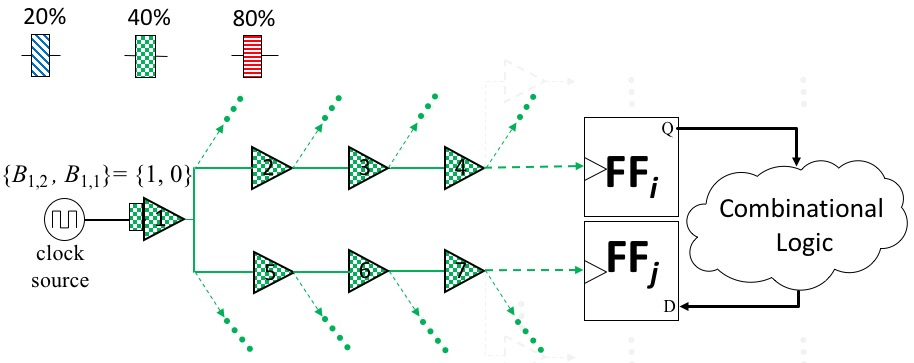
\includegraphics[width=0.9\columnwidth]{A_examlpe_of_DCC_placement1.png}
    }
    \hspace{1cm}
    \subfigure[Case 2-2: one DCC on one of the divergent clock paths, or class 3: two DCCs, one on each of the divergent clock paths]{
    	\label{fig:sub:dcci2}
        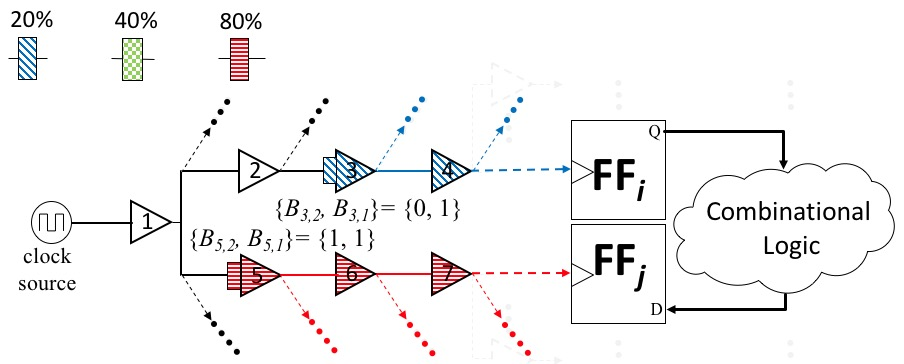
\includegraphics[width=0.9\columnwidth]{A_examlpe_of_DCC_placement2.png}
    }
    \caption{Examples of DCC insertion}
    \label{fig:dccinsert}
\end{figure*}
}

For example, in Figure~\ref{fig:sub:dcci2}, a 20\% DCC and an 80\% DCC are inserted at buffer 3 and buffer 6, respectively. Moreover, the buffer 5 is selected as the $V_{th}^h$ leader, denoted by a black flag, implying the $V_{th}$ of buffers 5, 6 and 7 are assigned to high $V_{th}$. Therefore, {\small $\left\{B_{3,3}, B_{3,2}, B_{3,1}\right\}$ = \{0, 0, 1\}}, {\small $\left\{B_{5,3}, B_{5,2}, B_{5,1}\right\}$ = \{1, 0, 0\}}, {\small $\left\{B_{6,3}, B_{6,2}, B_{6,1}\right\}$ = \{0, 1, 1\}}, and {\small $\left\{B_{p,3}, B_{p,2}, B_{p,1}\right\}$ = \{0, 0, 0\}} for $p$ = 1, 2, 4 or 7.

The 20\% DCC will mitigate the aging of buffer 3 and its downstream buffers, while the 80\% DCC will aggravate the aging of buffer 6 and its downstream buffers. It can be found that, if a DCC is deployed deep in the clock tree (i.e., close to the flip-flops), the count of affected buffers is limited and thus the overall impact of aging mitigation/aggravation on $C_i$/$C_j$ may be insignificant, diminishing the benefit from deploying DCCs for aging tolerance. Similarly, it can also be observed that, if we select a deep-located buffer as $V_{th}^h$ leader, the count of $V_{th}^h$ buffers is limited, also diminishing the benefit for aging tolerance. To avoid the phenomena, we set a rule of prohibiting DCC deployment and leader selection at a clock tree level larger/deeper than a specified boundary. This rule also greatly reduces the complexity of our SAT-based formulation because a significant fraction of buffers are excluded from being considered inserted DCC at their inputs and selected as $V_{th}^h$ buffer leader. For example, in Figure~\ref{fig:dcctype}, those dashed buffers and their downstream buffers are excluded. 

%(2) B
\subsection{DCC Constraints, Leader Constraints and Corresponding Clauses}
\label{subsec:dccccc}

Figure~\ref{fig:dcctype} shows a generalized example of DCC insertion for a pair of flip-flops (\ce{FF_i} and \ce{FF_j}) where there exist aging-critical paths from \ce{FF_i} to \ce{FF_j}. A path is defined as an aging-critical path if, in the presence of aging, it is possible to determine the clock period of the circuit. Every pair of flip-flops between which there exist aging-critical paths needs to be considered and here, we use this generalized example to illustrate our SAT-based formulation.

In Figure~\ref{fig:dcctype}, buffers 1 $\hyphen$ 7 are candidate locations for DCC insertion and according to the encoding scheme explained in Section~\ref{subsec:eddcd}, three Boolean variables are introduced for each of the seven buffers to encode eight possibilities of DCC insertion. Considering all seven buffers, there are a total of 16,384 (= $4^7$) possibilities for DCC insertions and 128 (= $2^7$) possibilities for leader selections, just for this pair of flip-flops. This makes the SAT-based formulation intractable due to the explosion of clause count. Therefore, we set up the following constraints on DCC insertion and the selection of $V_{th}^h$ buffer leader: 

{\noindent \textbf{\uline{DCC constraint: At most one DCC on a single clock path (from the clock source to one of the flip-flops)}}}

In order to ensure no more than one DCC on any clock path, we can use the Boolean variables introduced for DCC insertion, i.e., $B_{p,q} \left(1 \leq p \leq P, 1 \leq q \leq Q = \lceil \lg (N + 1) \rceil \right)$, to generate some clauses which suppress the occurrence of having two DCCs on a clock path. Consider buffer 2 (encoded by $\left\{B_{2,2}, B_{2,1}\right\}$) and buffer 3 (encoded by $\left\{B_{3,2}, B_{3,1}\right\}$) in Figure~\ref{fig:dcctype}. If there is a DCC at buffer 2 (i.e., $\{B_{2,2}, B_{2,1}\} \not\equiv \{0, 0\}$), then there must no DCC at buffer 3 (i.e., $\{B_{3,2}, B_{3,1}\} \equiv \{0, 0\}$), and vice versa. The constraint can be formally written as:
\begin{gather*}
\left(\{B_{2,2}, B_{2,1}\} \equiv \{0, 0\}\right) \lor \left(\{B_{3,2}, B_{3,1}\} \equiv \{0, 0\}\right)
\end{gather*}
Next, it can be translated into 4 CNF clauses:
\begin{equation*}
\begin{split}
(\neg B_{2,1}\lor\neg B_{3,1}) \land (\neg B_{2,1}\lor\neg B_{3,2}) \\
\land (\neg B_{2,2}\lor\neg B_{3,1}) \land (\neg B_{2,2}\lor\neg B_{3,2})
\end{split}
\end{equation*}

Any pair of buffers along a single clock path should be constrained in this way. Among buffers 1 $\hyphen$ 7 in Figure~\ref{fig:dcctype}, there are 12 pairs: $\langle1, 2\rangle$, $\langle1, 3\rangle$, $\langle1, 4\rangle$, $\langle1, 5\rangle$, $\langle1, 6\rangle$, $\langle1, 7\rangle$, $\langle2, 3\rangle$, $\langle2, 4\rangle$, $\langle3, 4\rangle$, $\langle5, 6\rangle$, $\langle5, 7\rangle$, $\langle6, 7\rangle$. Each pair translates to 4 clauses and a total of 48 clauses will be generated accordingly.
The corresponding clauses for leader constraints can also be generated in a similar manner. In the example, the 12 clauses are generated but are not shown in the paper due to brevity.

With DCC constraints and corresponding clauses, we can drastically reduce the possibilities of DCC insertions to be formulated. In the above example where the 48 clauses associated with DCC constraints are generated, the possibility count of DCC insertions drops from 16,384 to 103. In the next subsection, we describe what the 103 possibilities are and how they are translated into the final CNF representation.

{\noindent \textbf{\uline{Leader constraint: At most one clock buffer on a single clock path is selected as $V_{th}^h$ buffer leader}}}

To suppress the occurrence that, two buffers along a clock path are selected as $V_{th}^h$ buffer leaders, the associated 12 clauses can be generated in a similar manner, but they are not shown in the paper for brevity. Because of leader constraints and corresponding clauses, we can reduce the possibilities of leader selections to be formulated. Actually, the 12 clauses associated with leader constraints reduce the possibility count of leader selection from 128 to 17. In the next subsection, we describe what the 103 possibilities are and how they are translated into the final CNF representation.

%(3) C
\subsection{Timing Constraints and Corresponding Clauses}
\label{subsec:tccc}
Given a pair of flip-flops, if there exists one logic path between them, the timing (i.e. setup-time and hold-time) constraints must be met based on the inequalities~(\ref{eq:tsu}) and~(\ref{eq:th}). Different types of DCCs and $V_{th}^h$ buffer leaders reveal different influence on clock latency. Consider the lifespan specification of 10 years in Figure~\ref{fig:sub:dcci2}: the delay of each clock buffer is changed after 10 years. The clock latency of \ce{FF_i} (i.e., $C_i$) is the sum of clock buffer delays from clock source to \ce{FF_i}: \\
$C_i = \tau_1 + \tau_2 + \tau_3 + \tau_4 +\dotsb$ and \\
$C_j = \tau_1 + \tau_5 + \tau_6 + \tau_7 +\dotsb$, \mbox{\fontsize{9}{10.8}\selectfont where $\tau_k$ is the delay of buffer $k$.}\\
Consider aging effects on $C_i$ and $C_j$: \\
$C_{i\_aged} = 1.13 \times \left(\tau_1 + \tau_2\right) + 1.09 \times \left(\tau_3 + \tau_4 + \dotsb\right)$ and \\
$C_{j\_aged} = 1.13 \times \tau_1+ 1.16 \times \left( \tau_5 + \tau_6 + \tau_7 + \dotsb \right)$, where $C_{i\_aged}$ and $C_{j\_aged}$ denote aged $C_i$ and $C_j$, respectively.

Next, we apply Equations~(\ref{eq:tsu}) and~(\ref{eq:th}) to check whether timing constraints will be violated under this DCC deployment.\\ \\
\textbf{\uline{Timing constraint: No existence of timing violation}}

Given one clock period $T_c$ derived by binary search, one aging-critical path, and its associated clock network, all possible DCC deployments can be classified into 3 classes according to the number of DCCs used. Furthermore, due to the aforementioned DCC constraints, the SAT solver will only output a DCC deployment where there does not exist more than one DCC along any clock path. Thus, in the following discussion, the deployment with more than one DCC along a single clock path can be ignored. In each class, if the DCC deployment causes a timing violation within 10 years (i.e., the lifespan specification), then the deployment will be transformed into CNF clauses, such that the solver will not output the deployment as results. Here, we explain the generation of CNF clauses by using the example in Figure~\ref{fig:dccinsert}.

\begin{class}
\label{class:c1}
No DCC is inserted on either clock path

Consider the situation that no DCC is inserted at buffers 1 $\hyphen$ 7. If it causes a timing violation along the aging-critical path within 10 years, then the Boolean representation of the deployment,
{\fontsize{8}{8.4}
\begin{gather*}
\left(\{B_{1,2}, B_{1,1}\} \equiv \{0, 0\} \right) \land \left( \{B_{2,2}, B_{2,1}\} \equiv \{0, 0\} \right) \land \dotsb \\
\land \left( \{B_{7,2}, B_{7,1}\} \equiv \{0, 0\} \right),
\end{gather*}}
equivalent to the following CNF clause:
{\fontsize{8}{8.4}
\begin{gather*}
\left(B_{1,2} \lor B_{1,1} \lor B_{2,2} \lor B_{2,1} \lor \dotsb \lor B_{7,2} \lor B_{7,1} \right),
\end{gather*}}
should be generated such that the solver will not output the corresponding deployment in the result if the CNF is satisfiable. In this case, a total of 1 CNF clause is generated.
\end{class}
\begin{class}
\label{class:c2}
Inserting one DCC

This class can be further classified into 2 sub-classes based on the location of inserted DCCs. \\
\textit{Class 2-1:} Inserting one DCC on the common clock path

In Figure~\ref{fig:dccinsert}, buffer 1 is on the common clock path. Consider the DCC insertion shown in Figure~\ref{fig:sub:dcci1}: if the insertion of a 40\% DCC at buffer 1 causes a timing violation within 10 years, then the Boolean representation of the DCC deployment, {\fontsize{8}{8.4}$\left(\{B_{1,2}, B_{1,1}\} \equiv \{1, 0\} \right) \land \left( \{B_{2,2}, B_{2,1}\} \equiv \{0, 0\} \right) \land \dotsb \land \left( \{B_{7,2}, B_{7,1}\} \equiv \{0, 0\} \right)$}, equivalent to the following clause:  {\fontsize{8}{8.4}$\left(\neg B_{1,2} \lor B_{1,1} \lor B_{2,2} \lor B_{2,1} \lor \dotsb \lor B_{7,2} \lor B_{7,1} \right)$}, should be generated such that the solver will not output the deployment in the result if the CNF is satisfiable. Given that there are 3 choices of DCCs, a total of 3 CNF clauses will be generated in the worst case. \\
\textit{Class 2-2:} \mbox{\fontsize{9}{10.8}\selectfont Inserting one DCC on one of the divergent clock paths}

This class targets buffers 2, 3, 4, 5, 6, 7. If the insertion of a 20\% DCC at buffer 3 causes a timing violation within 10 years, then the Boolean representation of the DCC deployment,  {\fontsize{8}{8.4}$\left(\{B_{3,2}, B_{3,1}\} \equiv \{0, 1\} \right) \land \left( \{B_{1,2}, B_{1,1}\} \equiv \{0, 0\} \right) \land \dotsb \land \left( \{B_{7,2}, B_{7,1}\} \equiv \{0, 0\} \right)$}, equivalent to the following CNF clause:  {\fontsize{8}{8.4}$\left(B_{3,2} \lor \neg B_{3,1} \lor B_{1,2} \lor B_{1,1} \lor B_{2,2} \lor B_{2,1} \lor B_{3,2} \dotsb \lor B_{7,2} \lor B_{7,1} \right)$}, should be generated such that the solver will not output the deployment in the result if the CNF is satisfiable. This class includes 6 candidates: buffers 2, 3, 4, 5, 6, 7, and each has 3 choices of DCCs. Therefore, a total of 18 CNF clauses will be generated in the worst case.
\end{class}

\begin{class}
\label{class:c3}
Inserting two DCCs on two clock paths respectively

Given the DCC deployment in Figure~\ref{fig:sub:dcci2} (a 20\% DCC inserted at buffer 3 and a 80\% DCC inserted at buffer 6), if it causes a timing violation along the aging-critical path within 10 years, then the Boolean representation of the deployment, {\fontsize{8}{8.4}$\left(\{B_{3,2}, B_{3,1}\} \equiv \{0, 1\} \right) \land \left( \{B_{5,2}, B_{5,1}\} \equiv \{1, 1\} \right)$}, equivalent to the following CNF clause: {\fontsize{8}{8.4}$\left(B_{3,2} \lor \neg B_{3,1} \lor \neg B_{5,2} \lor \neg B_{5,1} \right)$}, should be generated such that the solver will not output the deployment in the result if the CNF is satisfiable.

Class 3 considers two buffer locations to insert DCCs, one among buffers \{2, 3, 4\} and the other one among buffers \{5, 6, 7\}; thus, there are totally 9 combinations of buffer locations. Each combination includes two buffers and thus 9 possibilities of choosing one specific DCC for each of the two buffers. Therefore, a total of 81 CNF clauses will be generated in the worst case.

Considering all of the above cases, a maximum number of 1 + 3 + 18 + 81 = 103 clauses can be derived. This is based on the existence of 48 clauses introduced in Section~\ref{subsec:dccccc}.

\end{class}

\begin{figure}
    \centering
    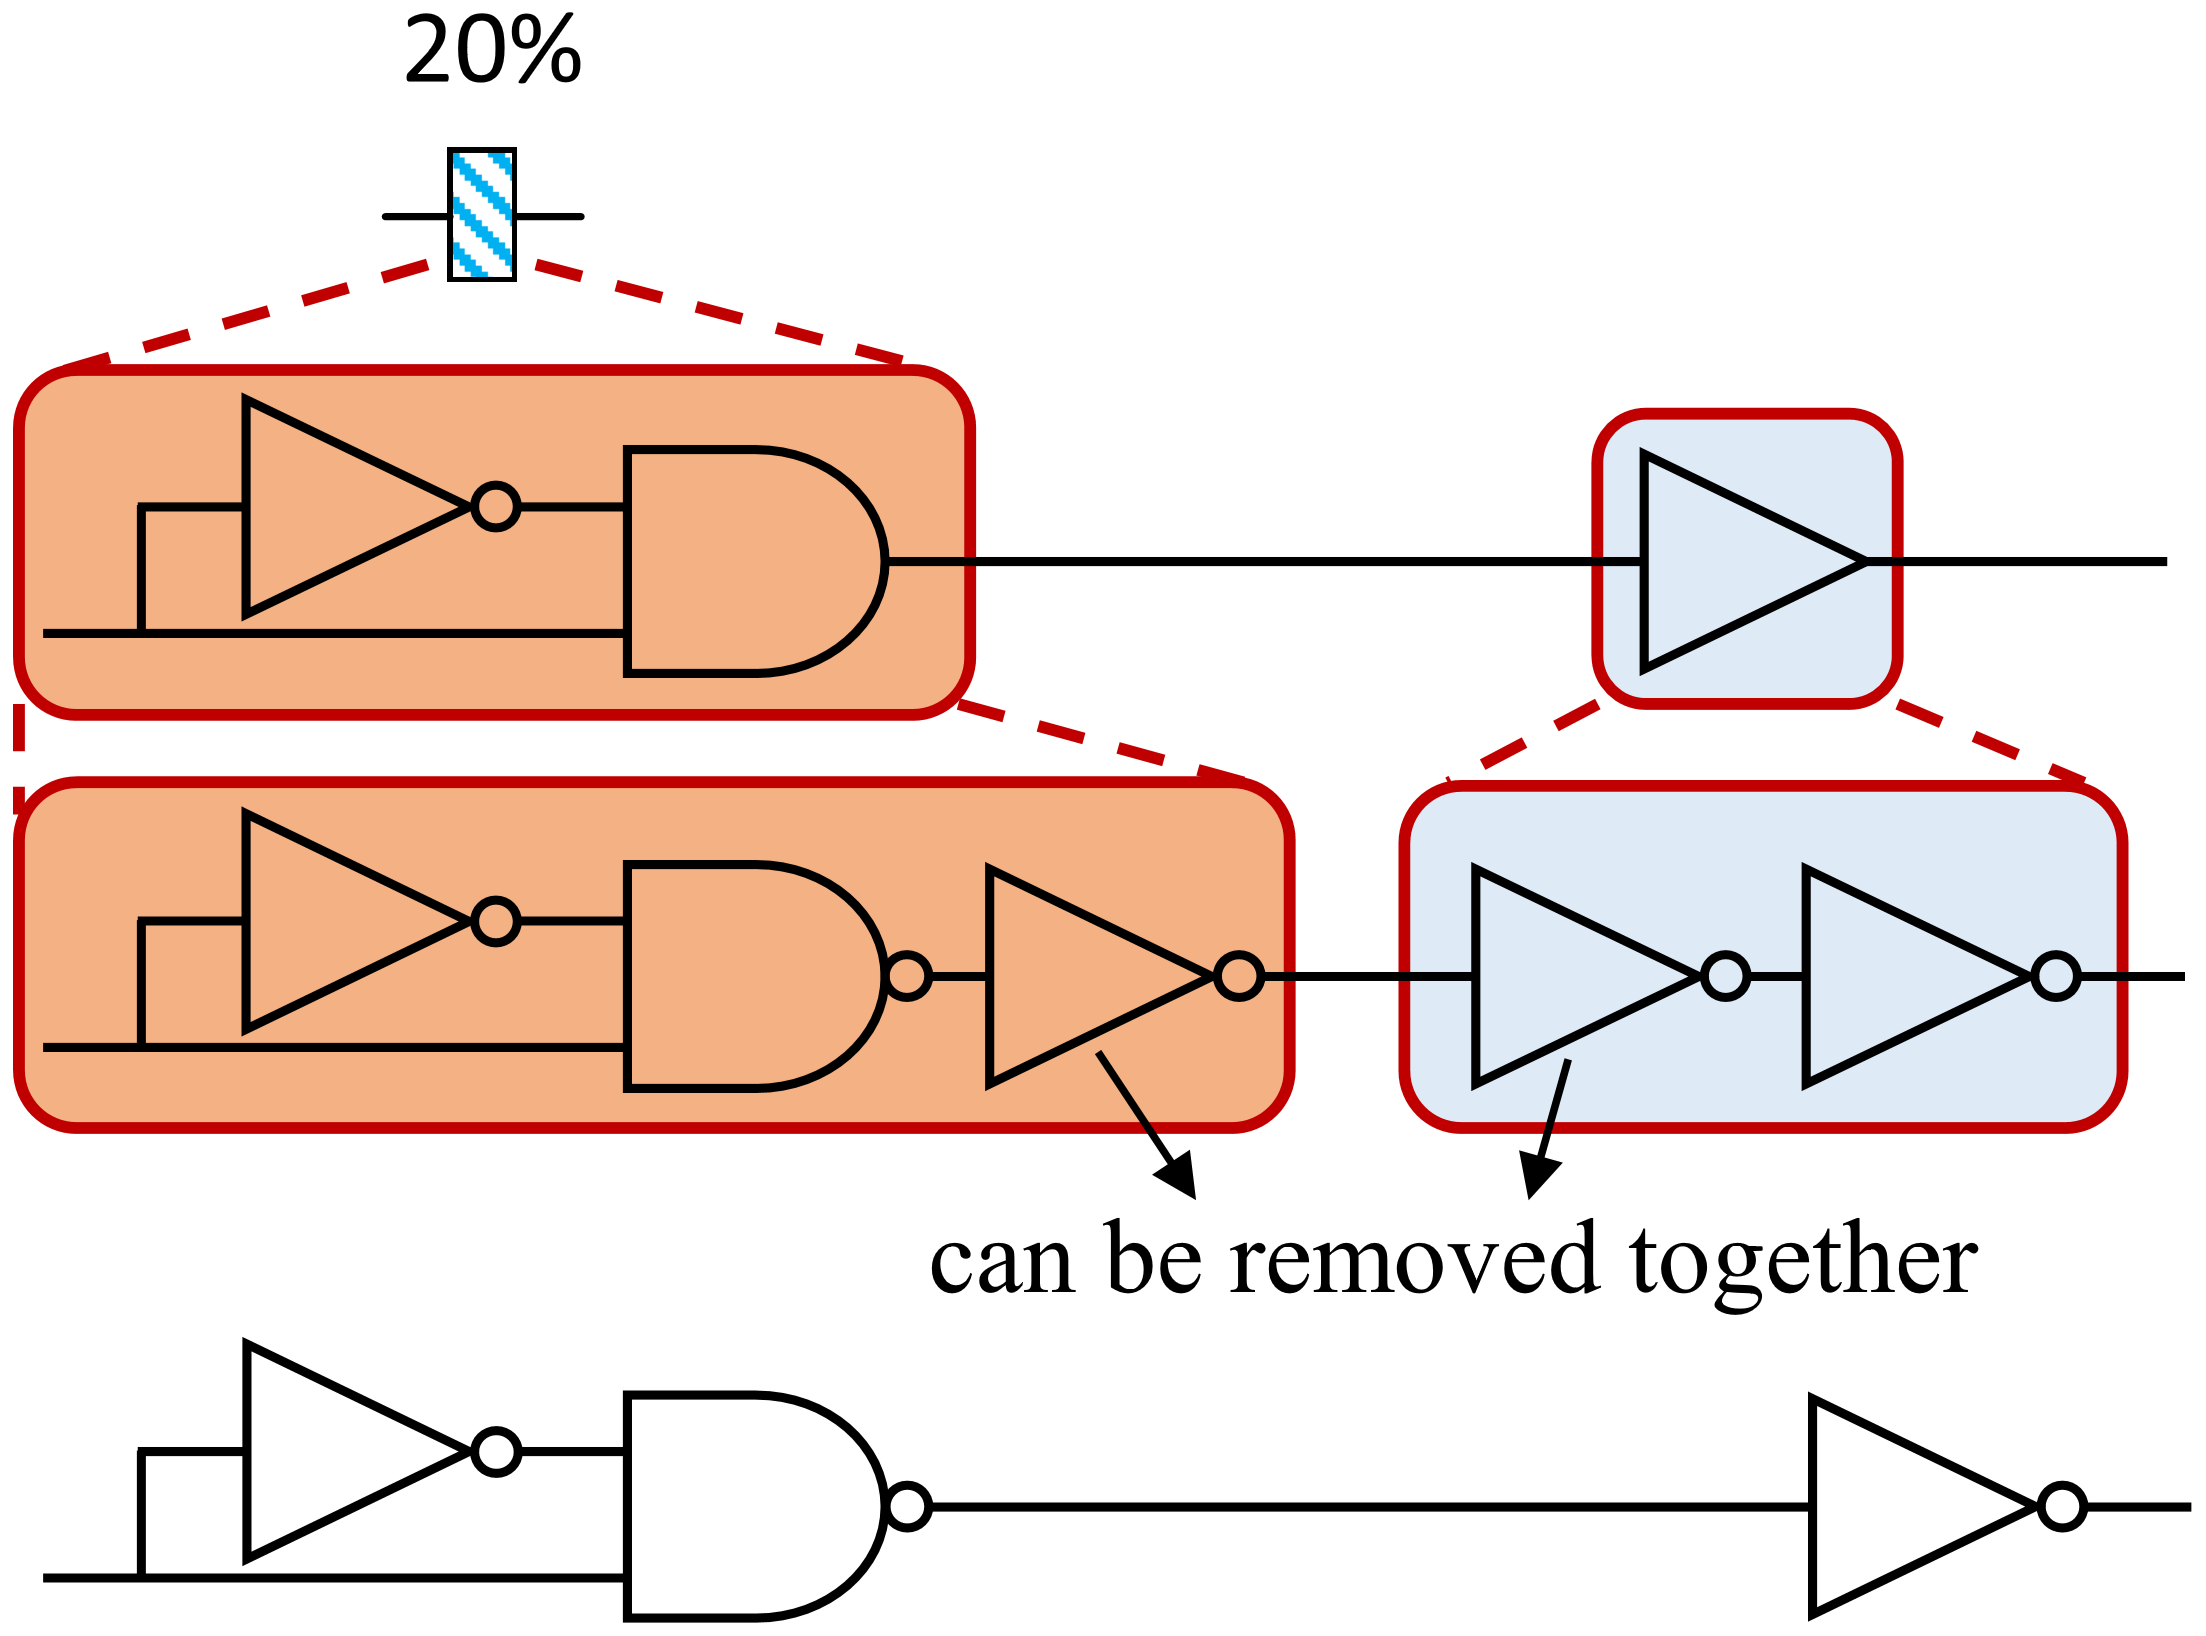
\includegraphics[width=0.5\columnwidth]{DCC_reduction.png}
    \caption{Practical considerations for DCC insertion}
    \label{fig:dccreduc}
\end{figure}

\subsection{Practical Considerations}
\label{subsec:tpc}
The diagram on the top of Figure~\ref{fig:dccreduc} shows the primitive design of a DCC, consisting of an inverter and an AND gate. In practice, the AND gate is implemented by a NAND gate feeding an inverter. As mentioned earlier, when inserting a DCC, it is inserted at the input of a buffer, which is a pair of inverters in practice. Therefore, we can actually use the diagram on the bottom of Figure~\ref{fig:dccreduc} to realize the insertion of a DCC. More specifically, we use it as a new cell to \enquote{replace} a buffer when a DCC is needed. By doing so, the cost of a single DCC can be significantly reduced and not much more expensive than the cost of inserting a buffer for clock skew scheduling. 